%----------------------------------------------------------------------
\chapter{Funcionalidades}
Assim como ilustra a \autoref{fig_diag_virado}, o usuário pode acessar o site sem efetuar cadastro ou login. Dessa forma, seu acesso será restrito apenas a timeline (\autoref{fig_timeline}) e aos perfis dos animais (\autoref{fig_perfil}), precisando estar logado em uma conta para acessar outros recursos, como doar e/ou adotar um animal.

% DELIMITAR DISTANCIA -------------------------------------------------
\section{Delimitar distância}
Após realizar o cadastro, o sistema deve pedir a permissão do usuário para acessar sua localização. Dessa forma, será possível encontrar os animais mais próximos a ele e delimitar a exibição por proximidade, evitando problemas de deslocamento em maiores distâncias, que poderiam atrapalhar, ou até mesmo impedir a adoção.
%----------------------------------------------------------------------

% ADOTAR --------------------------------------------------------------
\section{Adotar}
Para adotar um animal, o usuário, já cadastrado, deve preencher um formulário de adoção, como na \autoref{fig_formulario}, informando dados pessoais importantes para o doador do animal. Em seguida, deve realizar a procura de animais que pode ser feita de três maneiras diferentes. São elas: 
\begin{itemize}
\item Manual: o usuário pode procurar pelo animal que mais lhe agradar através da timeline, observando a foto do animal e as informações primárias disponíveis nela;
\item Com filtros: a procura pode ser feita com o auxílio de filtros que produzem resultados delimitados através das preferências do usuário;
\item Combinação perfeita: através desse recurso, o usuário não precisa procurar um animal compatível com suas preferências, o sistema faz isso para ele, comparando algumas das informações dadas por ele no formulário de adoção e as de cada um dos animais informadas no momento do cadastro (\autoref{fig_cad_animal}).
\end{itemize}
%----------------------------------------------------------------------

% MATCH ---------------------------------------------------------------
\section{Match}
Ao encontrar o animal que deseja adotar, o usuário tem a opção de curtir o perfil, o que gera uma notificação para o doador desse respectivo animal, que poderá retribuir a curtida ou não. Caso isso ocorra, acontecerá o match, que colocará os dois usuários (adotante e doador) em contato através do chat do site e mudará o status do animal de "disponível" para "em processo de adoção", impossibilitando outros adotantes de curtirem esse animal.
Enquanto um animal está em processo de adoção, outros usuários ficam impossibilitados de curtir ele, mas, podem entrar em uma fila de espera para match no caso da adoção com o adotante da vez não acontecer.
%----------------------------------------------------------------------

% MONITORAMENTO DE CHAT -----------------------------------------------
\section{Monitorar chat}
Durante o processo de adoção, enquanto os usuários adotante e doador estiverem em contato no chat, as mensagens trocadas serão monitoradas, de forma que, em caso de usarem palavras registradas no sistema como impróprias, o usuário que a enviou terá cometido uma infração. Caso o mesmo usuário cometa três infrações, sua conta será banida temporariamente e, e caso uma mesma conta seja banida três vezes, será excluida permanentemente.
%----------------------------------------------------------------------
\begin{figure}[htb]
    \centering
	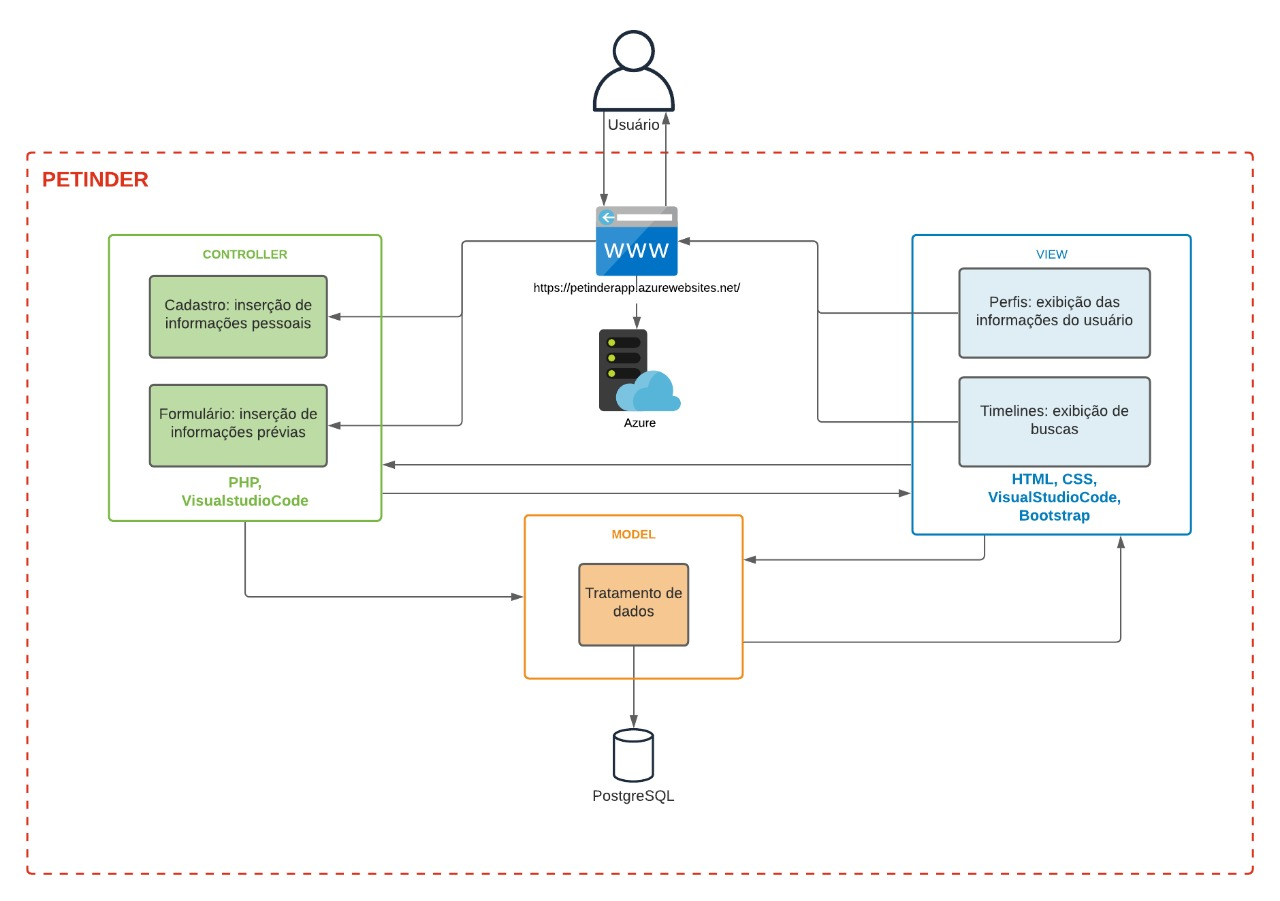
\includegraphics[width=1\textwidth]{imagens/diagrama_de_arquitetura.jpg}
	\caption{\label{fig_diagrama}Diagrama de arquitetura do sistema}
	\fonte{Elaborada pelos autores}
\end{figure}


%--------------------------------------------------------------------------
\chapter{Tecnologias}
As tecnologias que serão utilizadas durante o ano na disciplina, não apenas no desenvolvimento da aplicação, mas também na redação da documentação, e no registro de atividades e entregas, serão:
\begin{itemize}
\item Front-end: HTML5, CSS3 e JavaScript;
\item Framework: Bootstrap 4;
\item Back-end: PHP;
\item Banco de dados: PostgreSQL com a extensão geoespacial PosGIS;
\item IDE: Visual Studio Code e Eclipse;
\item Documentos: \LaTeX;
\item Controle de Versão: Subversion;
\item Gource;
\end{itemize}

%--------------------------------------------------------------------------
\chapter{Equipe}
A equipe TI TI TI é composta por seis integrantes e possui esse nome como uma referência a relação do nome da novela da Rede Globo Ti-Ti-Ti e a sigla da área do conhecimento Tecnologia da Informação (TI), e deve ser lido como uma tripla repetição da sigla. A divisão de tarefas da equipe no desenvolvimento do PETINDER pode ser observada no \autoref{quadro}.

\begin{quadro}[htb]
\centering
\ABNTEXfontereduzida
\caption[Divisão de Tarefas]{Divisão de Tarefas}
\label{quadro}
\begin{tabular}{|c|c|c|c|c|c|}
  \hline
   \thead{Integrante} & \thead{Front-end}  & \thead{Back-end}  & \thead{Documentação} & \thead{Mídias} & \thead{Banco de dados} \\
    \hline
    Brenda & X & X &  &  & X \\
    \hline
    Cecília &  &  & X &  &  \\
    \hline
    Eduarda & X &  &  & X &  \\
    \hline
    Fernanda &  &  & X &  & \\
    \hline
    Gabriela &  &  & X &  & \\
    \hline
    Giovana & X  & X &  &  & X\\
    \hline
\end{tabular}
\legend{Fonte: Elaborado pelos autores}
\end{quadro}
%--------------------------------------------------------------------------
%--------------------------------------------------------------------------
%----------------------------------------------------------------------